\chapter{UJI COBA DAN EVALUASI}\label{chap:uji-coba-eval}

\tab Bab ini membahas hasil uji coba aplikasi yang telah dirancang dan diimplementasikan. Uji coba dilakukan untuk mengetahui kinerja aplikasi dengan lingkungan uji coba yang telah ditentukan.

\section{Lingkungan Uji Coba}

Lingkungan pengujian menggunakan komponen-komponen yang terdiri dari:

\begin{enumerate}
	\item \textit{Processor} Intel(R) Core(TM) i3-5010U CPU @ 2.10GHz x 4
	\item RAM 6 GB
\end{enumerate}

Semua pengujian menggunakan Memory Heap pada JVM sebanyak 4 GB (dengan opsi -Xmx4g).

\section{Data Uji Coba}

\tab Terdapat tiga jenis data yang akan digunakan dalam pengujian Tugas Akhir ini. Tiga jenis data tersebut terdiri dari data \textit{independent}, data \textit{anticorrelated}, dan data \textit{correlated}.

\subsection{Data \textit{Independent} (IND)}

\tab Data \textit{independent} adalah sebuah data buatan dengan cara melakukan \textit{random} secara utuh dengan jumlah yang telah ditentukan.

\subsection{Data \textit{Anticorrelated} (ANT)}

\tab Data \textit{anticorrelated} adalah data yang memiliki hubungan negatif. Artinya, jika suatu nilai suatu atribut bertambah, maka atribut lain berkurang dengan rasio yang sama. Data \textit{anticorrelated} ini memungkinkan setiap objek tidak mendominasi dan didominasi oleh objek lain.

\subsection{Data \textit{Correlated} (COR)}
\tab Data \textit{correlated} adalah data yang memiliki hubungan erat. Dalam artian, jika nilai suatu atribut bertambah, maka atribut lain juga bertambah dengan rasio yang sama. Dalam kasus ini, suatu objek pasti mendominasi dan didominasi objek yang lain.

\section{Skenario Uji Coba} \label{skenarioujicoba}

\tab Untuk menguji \textit{performance} dari algoritme yang diusulkan, kami mengujinya dengan beberapa variasi pada faktor-faktor yang mempengaruhi jalannya algoritme, yaitu: jumlah objek, jumlah sel grid, jumlah \textit{instance} tiap objek, dan jarak $ d_\varepsilon $. Berikut kami sajikan tabel variasi faktor-faktor yang disebutkan beserta nilai \textit{default}.

\begin{table}[!htb]
	\centering
	\begin{tabular}{| l | l | l |}
		\hline
		\textbf{Parameter} & \textbf{\textit{Default}} & \textbf {Rentang} \\ \hline
		Jumlah sel grid & $ 256^2 $ & $ 32^2 $, $ 64^2 $, $ 128^2 $, $ 256^2 $, $ 512^2 $ \\ \hline
		Jumlah objek (K) & 5 & 0.1, 1, 5, 10, 20 \\ \hline
		Jumlah \textit{instance} tiap objek & 50 & 10, 50, 100, 200, 400 \\ \hline
		$ d_\varepsilon $ (\%) & 1 & 0.1, 0.5, 1, 2, 3 \\ \hline
		Dimensi data & 2 & 2, 3, 4, 5, 6 \\ \hline
	\end{tabular}
	\caption{Atribut dari objek
		\label{tab:uji}}
\end{table}

\tab Uji coba dilakukan pada peta California\cite{ontrip} dengan irisan garis lintang antara 32.0 hingga 37.0 dan garis bujur antara -120.0 hingga -114.0. Pada koordinat tersebut didapat \textit{node} sebanyak 8716 dan \textit{edge} sebanyak 9077.

\subsection{Skenario Uji Coba \textit{Performance}}
\tab Pada sub-bab ini, kami menampilkan tabel uji \textit{performance} dalam bentuk grafik. Perlu diperhatikan bahwa beberapa grafik pada bab ini menggunakan skala logaritma pada sumbu \textit{y}. Uji coba dilakukan dengan membandingkan dengan metode \textit{naive}. Metode \textit{naive} mencari jarak terdekat setiap \textit{node} ketika terdapat objek baru masuk pada sistem dan memasukkan objek pada \textit{node} yang berjarak kurang dari $ d_\varepsilon $. Metode ini juga tidak menggunakan penanda \textit{isImpossible}, artinya, jika terdapat objek baru masuk pada suatu \textit{node}, maka metode ini membandingkan objek tersebut dengan semua objek yang ada.

\subsubsection{Skenario Uji Coba \textit{Performance} Terhadap Perubahan Jumlah Sel}

\tab Perubahan jumlah sel pada grid indeks tidak memberikan pengaruh banyak pada waktu komputasi dan penggunaan memori. Hal tersebut dikarenakan, jika jumlah sel sedikit, maka proses pengambilan data semakin cepat. Tetapi di sisi lain, pemrosesan data melambat karena objek yang dimuat semakin banyak. Jika jumlah sel banyak, pengambilan data semakin lama, tetapi pemrosesan data semakin cepat karena objek yang dimuat semakin sedikit.

\begin{figure}[H]
	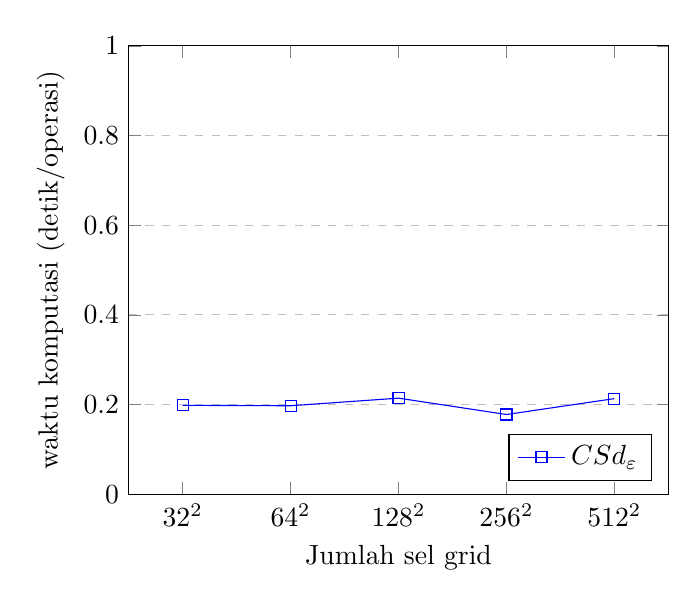
\begin{tikzpicture}
	\begin{axis}[
	xlabel={Jumlah sel grid},
	ylabel={waktu komputasi (detik/operasi)},
	ymin=0, ymax=1,
	xmin=0, xmax=10,
	xtick={1, 3, 5, 7, 9},
	xticklabels={$ 32^2 $, $ 64^2 $, $ 128^2 $, $ 256^2 $, $ 512^2 $},
	legend pos=south east,
	ymajorgrids=true,
	grid style=dashed,
	]
	
	\addplot[
	color=blue,
	mark=square,
	]
	coordinates {
		(1, 0.198035104400913)(3, 0.19713375528914)(5, 0.214094556217187)(7, 0.177597533827906)(9, 0.213052689078089)
	};
	\addlegendentry{$ CSd_\varepsilon $}
	
	\end{axis}
	\end{tikzpicture}
	\caption{Pengaruh jumlah sel terhadap waktu komputasi tiap operasi dalam satuan detik}\label{fig:uji-g}
\end{figure}

\tab Jumlah sel tidak banyak mempengaruhi penggunaan memori dan waktu komputasi. Hal ini dikarenakan adanya \textit{trade-off} antara proses memuat data dengan komputasi. Grid indeks yang memiliki sel sedikit menjadikan data yang dimuat lebih banyak sehingga menjadikan data yang diproses labih banyak. Tetapi di sisi lain, sistem tidak banyak mencari data secara berulang-ulang karena setiap sel sudah mengaver area yang besar. Sedangkan grid indeks yang memiliki sel yang banyak menjadikan proses komputasi lebih efisien karena melibatkan data yang lebih sedikit. Tetapi di sisi lain, sistem harus melakukan pencarian data berulang-ulang karena sedikitnya data yang didapat pada setiap sel.

\begin{figure}[H]
	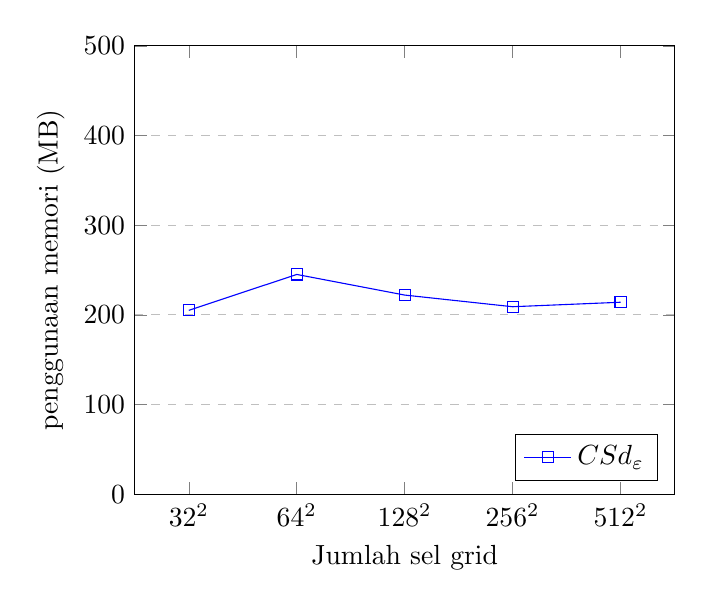
\begin{tikzpicture}
	\begin{axis}[
	xlabel={Jumlah sel grid},
	ymin=0, ymax=500,
	ylabel={penggunaan memori (MB)},
	xmin=0, xmax=10,
	xtick={1, 3, 5, 7, 9},
	xticklabels={$ 32^2 $, $ 64^2 $, $ 128^2 $, $ 256^2 $, $ 512^2 $},
	legend pos=south east,
	ymajorgrids=true,
	grid style=dashed,
	]
	
	\addplot[
	color=blue,
	mark=square,
	]
	coordinates {
		(1, 205)(3, 245)(5, 222)(7, 209)(9, 214)
	};
	\addlegendentry{$ CSd_\varepsilon $}
	
	\end{axis}
	\end{tikzpicture}
	\caption{Pengaruh jumlah sel grid terhadap penggunaan memori dalam satuan megabita}\label{fig:uji-g-mem}
\end{figure}

\subsubsection{Skenario Uji Coba \textit{Performance} Terhadap Perubahan Jumlah Objek}
\tab Penggunaan waktu CPU pada algoritme $ CSd_\varepsilon-SQ$ jauh mengungguli algoritme \textit{naive}. Hal ini dikarenakan algoritme \textit{naive} menghitung jarak semua \textit{node} dengan objek yang masuk menggunakan \textit{shortest-path}, sedangkan $ CSd_\varepsilon-SQ $ hanya menggunakan \textit{node} yang diperlukan dan $ CSd_\varepsilon-SQ $ tidak menggunakan algoritme \textit{shortest-path}.

\begin{figure}[H]
	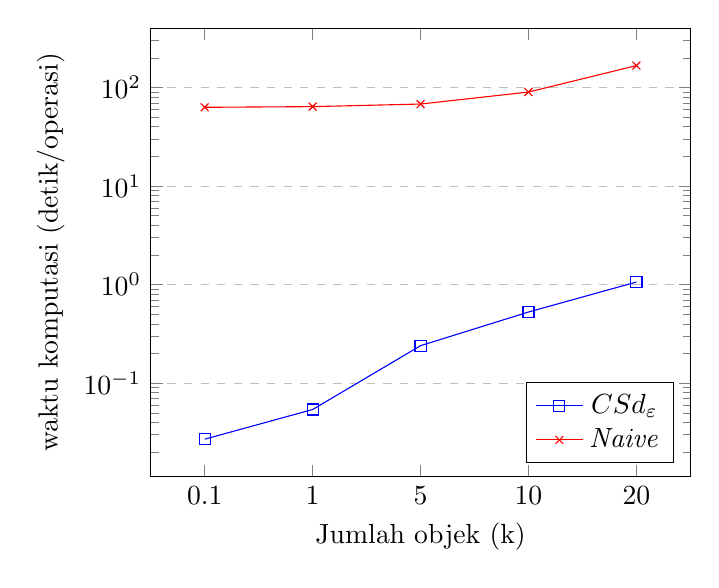
\begin{tikzpicture}
	\begin{axis}[
	xlabel={Jumlah objek (k)},
	ymode=log,
	ylabel={waktu komputasi (detik/operasi)},
	xmin=0, xmax=10,
	xtick={1, 3, 5, 7, 9},
	xticklabels={0.1, 1, 5, 10, 20},
	legend pos=south east,
	ymajorgrids=true,
	grid style=dashed,
	]
	
	\addplot[
	color=blue,
	mark=square,
	]
	coordinates {
		(1,0.027)(3, 0.054)(5, 0.24)(7, 0.527)(9, 1.062)
	};
	\addlegendentry{$ CSd_\varepsilon $}
	
	\addplot[
	color=red,
	mark=x,
	]
	coordinates {
		(1,63)(3, 64)(5, 68)(7, 90)(9, 167)
	};
	\addlegendentry{\textit{Naive}}
	
	\end{axis}
	\end{tikzpicture}
	\caption{Pengaruh jumlah objek terhadap waktu komputasi tiap operasi dalam satuan detik}\label{fig:uji-n}
\end{figure}

\tab Ketika jumlah objek bertambah, waktu pemrosesan juga bertambah, hal ini dikarenakan bertambahnya objek yang terdapat pada \textit{node}. Dengan bertambahnya objek pada \textit{node}, algoritme perlu membandingkan dengan objek yang lebih banyak untuk mencari probabilitas masing-masing objek menjadi \textit{SP}.

\begin{figure}[H]
	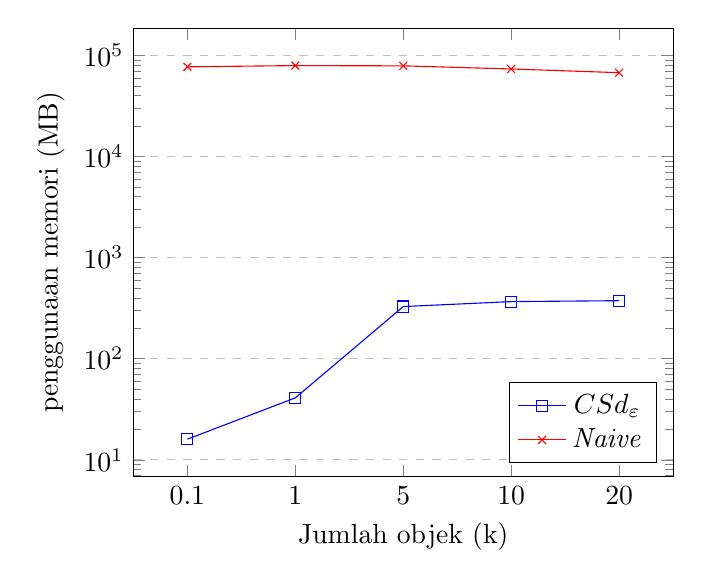
\begin{tikzpicture}
	\begin{axis}[
	xlabel={Jumlah objek (k)},
	ymode=log,
	ylabel={penggunaan memori (MB)},
	xmin=0, xmax=10,
	xtick={1, 3, 5, 7, 9},
	xticklabels={0.1, 1, 5, 10, 20},
	legend pos=south east,
	ymajorgrids=true,
	grid style=dashed,
	]
	
	\addplot[
	color=blue,
	mark=square,
	]
	coordinates {
		(1, 16)(3, 41)(5, 328)(7, 367)(9, 375)
	};
	\addlegendentry{$ CSd_\varepsilon $}
	
	\addplot[
	color=red,
	mark=x,
	]
	coordinates {
		(1, 77062)(3, 79292)(5, 78801)(7, 73392)(9, 67442)
	};
	\addlegendentry{\textit{Naive}}
	
	\end{axis}
	\end{tikzpicture}
	\caption{Pengaruh jumlah objek terhadap penggunaan memori dalam satuan megabita}\label{fig:uji-n-mem}
\end{figure}

\tab Terkait penggunaan memori, metode \textit{naive} membutuhkan memori yang sangat banyak karena banyaknya \textit{node} yang perlu diproses menggunakan algoritme \textit{shortest-path}. Sedangkan metode $ CSd_\varepsilon-SQ$ membutuhkan memori yang tidak banyak karena hanya menggunakan data \textit{node} yang diperlukan saja dengan struktur grid.

\subsubsection{Skenario Uji Coba \textit{Performance} Terhadap Perubahan Jumlah \textit{Instance} pada Objek}
\tab Jumlah \textit{instance} pada objek mempengaruhi waktu komputasi dan penggunaan memori. Hal ini dikarenakan proses penghitungan probabilitas melibatkan \textit{instances} di objek. Dari sisi memori, banyaknya \textit{instance} membuat sistem harus mengalokasikan memori lebih untuk proses penyimpanan dan komputasi.

\begin{figure}[H]
	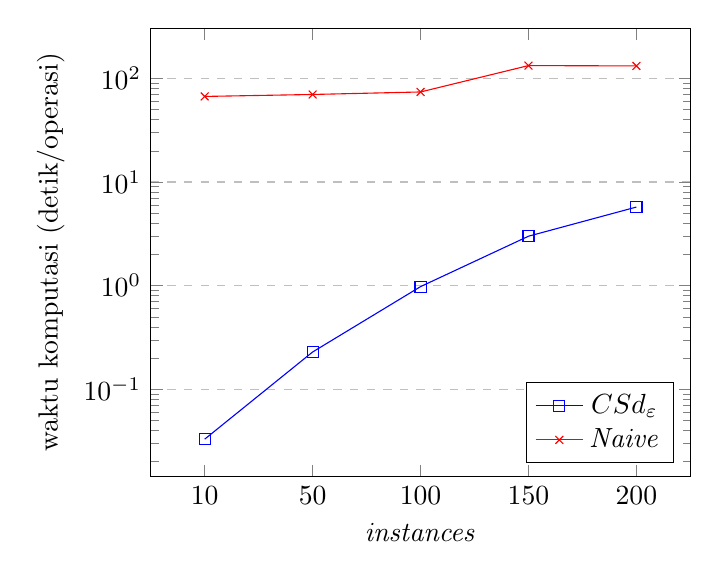
\begin{tikzpicture}
	\begin{axis}[
	xlabel={\textit{instances}},
	ymode=log,
	ylabel={waktu komputasi (detik/operasi)},
	xmin=0, xmax=10,
	xtick={1, 3, 5, 7, 9},
	xticklabels={10, 50, 100, 150, 200},
	legend pos=south east,
	ymajorgrids=true,
	grid style=dashed,
	]
	
	\addplot[
	color=blue,
	mark=square,
	]
	coordinates {
		(1, 0.033)(3, 0.229)(5, 0.979)(7, 3)(9, 5.736)
	};
	\addlegendentry{$ CSd_\varepsilon $}
	
	\addplot[
	color=red,
	mark=x,
	]
	coordinates {
		(1, 67)(3, 70)(5, 74)(7, 133)(9, 132)
	};
	\addlegendentry{\textit{Naive}}
	
	\end{axis}
	\end{tikzpicture}
	\caption{Pengaruh jumlah \textit{instance} terhadap waktu komputasi tiap operasi dalam satuan detik}\label{fig:uji-np}
\end{figure}

\tab Pada metode \textit{naive}, objek perubahan waktu komputasi terlihat ketika jumlah \textit{instance} diatas 100. Hal ini dikarenakan waktu komputasi lebih banyak digunakan untuk penghitungan jarak terpendek dari setiap \textit{node} ke objek, sehingga jumlah \textit{instance} yang sedikit tidak berpengaruh banyak terhadap waktu komputasi.

\begin{figure}[H]
	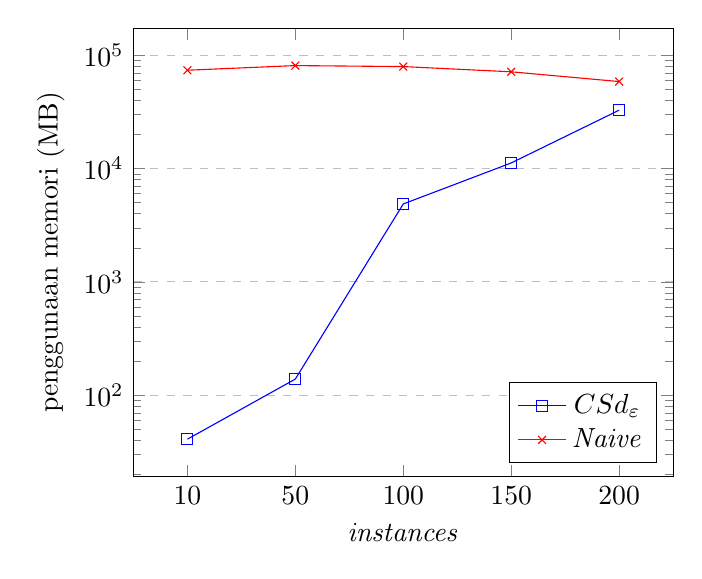
\begin{tikzpicture}
	\begin{axis}[
	xlabel={\textit{instances}},
	ymode=log,
	ylabel={penggunaan memori (MB)},
	xmin=0, xmax=10,
	xtick={1, 3, 5, 7, 9},
	xticklabels={10, 50, 100, 150, 200},
	legend pos=south east,
	ymajorgrids=true,
	grid style=dashed,
	]
	
	\addplot[
	color=blue,
	mark=square,
	]
	coordinates {
		(1, 41)(3, 139)(5, 4874)(7, 11213)(9, 32760)
	};
	\addlegendentry{$ CSd_\varepsilon $}
	
	\addplot[
	color=red,
	mark=x,
	]
	coordinates {
		(1, 73772)(3, 81068)(5, 79448)(7, 71448)(9, 58597)
	};
	\addlegendentry{\textit{Naive}}
	
	\end{axis}
	\end{tikzpicture}
	\caption{Pengaruh jumlah \textit{instance} terhadap penggunaan memori dalam satuan megabita}\label{fig:uji-np-mem}
\end{figure}

\subsubsection{Skenario Uji Coba \textit{Performance} Terhadap Perubahan Panjang Jarak Maksimal $ d_\varepsilon $}
\tab Jarak $ d_\varepsilon $ sangat mempengaruhi \textit{performance} karena $ d_\varepsilon $ menentukan jarak terjauh \textit{node} yang dapat menyimpan objek baru. Dengan bertambahnya nilai $ d_\varepsilon $, objek dapat menjangkau lebih banyak \textit{node}. Dengan demikian, objek yang ditampung pada \textit{node} menjadi semakin banyak. Dengan semakin banyaknya objek, proses penghiungan probabilitas \textit{skyline} menjadi semakin lama karena harus menghitung banyak objek. Pada $ CSd_\varepsilon-SQ$, semakin besar nilai $ d_\varepsilon $, semakin banyak grid yang diakses sehingga membutuhkan waktu yang lebih banyak. Pada metode \textit{naive}, terdapat perubahan waktu komputasi yang signifikan ketika nilai $ d_\varepsilon $ diatas 1.

\begin{figure}[H]
	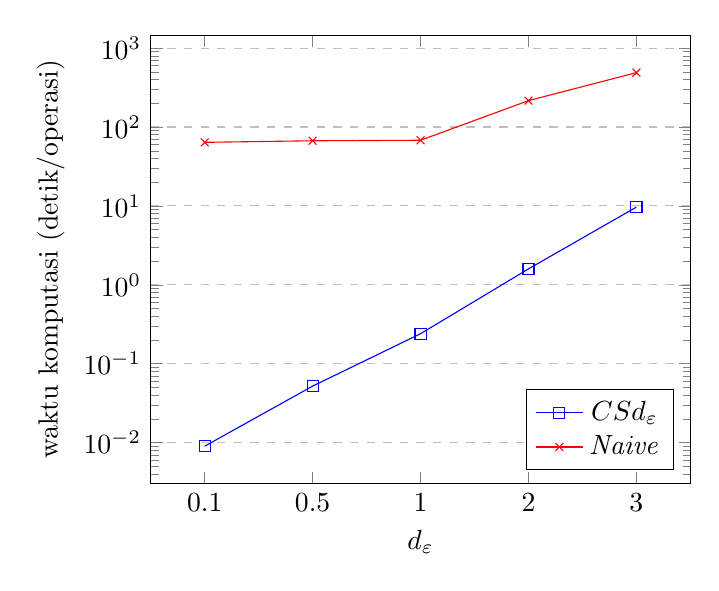
\begin{tikzpicture}
	\begin{axis}[
	xlabel={$ d_\varepsilon $},
	ymode=log,
	ylabel={waktu komputasi (detik/operasi)},
	xmin=0, xmax=10,
	xtick={1, 3, 5, 7, 9},
	xticklabels={0.1, 0.5, 1, 2, 3},
	legend pos=south east,
	ymajorgrids=true,
	grid style=dashed,
	]
	
	\addplot[
	color=blue,
	mark=square,
	]
	coordinates {
		(1, 0.009)(3, 0.052)(5, 0.24)(7, 1.592)(9, 9.667)
	};
	\addlegendentry{$ CSd_\varepsilon $}
	
	\addplot[
	color=red,
	mark=x,
	]
	coordinates {
		(1, 64)(3, 67)(5, 68)(7, 216)(9, 490)
	};
	\addlegendentry{\textit{Naive}}
	
	\end{axis}
	\end{tikzpicture}
	\caption{Pengaruh $ d_\varepsilon $ terhadap waktu komputasi tiap operasi dalam satuan detik}\label{fig:uji-d}
\end{figure}

\tab Penggunaan memori sangat tergantung dari jumlah objek yang diproses. Nilai $ d_\varepsilon $ yang besar menjadikan objek yang diproses semakin banyak karena setiap \textit{node} memiliki jangkauan yang lebih jauh. Banyaknya objek yang diproses menjadikan penggunaan memori semakin besar.

\begin{figure}[H]
	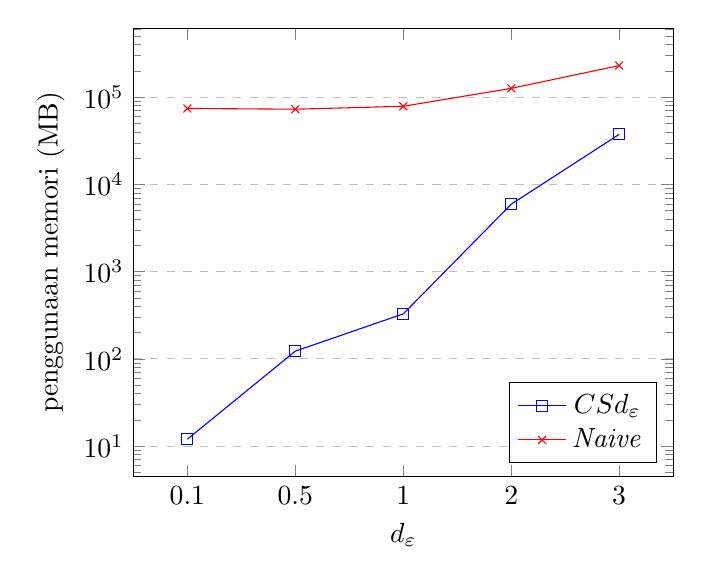
\begin{tikzpicture}
	\begin{axis}[
	xlabel={$ d_\varepsilon $},
	ymode=log,
	ylabel={penggunaan memori (MB)},
	xmin=0, xmax=10,
	xtick={1, 3, 5, 7, 9},
	xticklabels={0.1, 0.5, 1, 2, 3},
	legend pos=south east,
	ymajorgrids=true,
	grid style=dashed,
	]
	
	\addplot[
	color=blue,
	mark=square,
	]
	coordinates {
		(1, 12)(3, 122.7)(5, 328)(7, 5932)(9, 37507)
	};
	\addlegendentry{$ CSd_\varepsilon $}
	
	\addplot[
	color=red,
	mark=x,
	]
	coordinates {
		(1, 74387)(3, 72904)(5, 78801)(7, 126323)(9, 230699)
	};
	\addlegendentry{\textit{Naive}}
	
	\end{axis}
	\end{tikzpicture}
	\caption{Pengaruh $ d_\varepsilon $ terhadap penggunaan memori dalam satuan megabita}\label{fig:uji-d-mem}
\end{figure}
\subsubsection{Skenario Uji Coba \textit{Performance} Terhadap Perubahan Dimensi Data}

\tab Dimensi dari \textit{uncertian data} tidak banyak mempengaruhi \textit{performance} dari algoritma. Pada Gambar \ref{fig:uji-dim}, waktu komputasi pada algoritma $ CSd_\varepsilon $ cenderung turun. Hal tersebut dikarenakan antar objek tidak banyak yang mendominasi atau didominasi karena semakin banyaknya variabel yang perlu dibandingkan. Sebagai imbasnya, penggunaan memori semakin sedikit karena proses komputasi semakin sedikit.

\begin{figure}[H]
	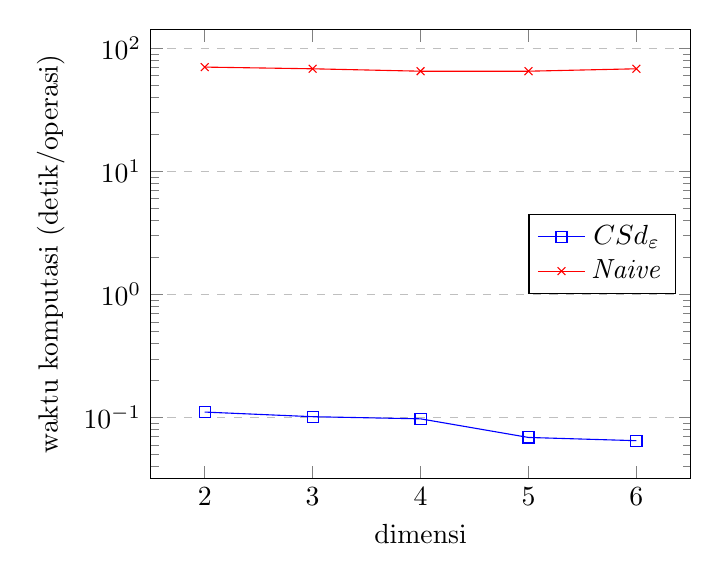
\begin{tikzpicture}
	\begin{axis}[
	xlabel={dimensi},
	ymode=log,
	ylabel={waktu komputasi (detik/operasi)},
	xmin=0, xmax=10,
	xtick={1, 3, 5, 7, 9},
	xticklabels={2, 3, 4, 5, 6},
	legend style={at={(0.7,0.5)},anchor=west},
	ymajorgrids=true,
	grid style=dashed,
	]
	
	\addplot[
	color=blue,
	mark=square,
	]
	coordinates {
		(1, 0.111)(3, 0.1018)(5, 0.0978)(7, 0.06906)(9, 0.065)
	};
	\addlegendentry{$ CSd_\varepsilon $}
	
	\addplot[
	color=red,
	mark=x,
	]
	coordinates {
		(1, 70.194)(3, 68)(5, 65)(7, 65)(9, 68)
	};
	\addlegendentry{\textit{Naive}}
	
	\end{axis}
	\end{tikzpicture}
	\caption{Pengaruh dimensi terhadap waktu komputasi tiap operasi dalam satuan detik}\label{fig:uji-dim}
\end{figure}

\tab Secara umum objek yang memiliki semakin banyak dimensi menjadikan objek tersebut semakin sedikit \textit{overlap}-nya dengan objek lain. Pada algoritma ini, proses penghitungan \textit{skyline} hanya dilakukan pada objek-objek yang overlap dengan objek yang dicari probabilitasnya. Dengan demikian, semakin banyak dimensi menjadikan waktu komputasi semakin kecil.

\tab Pengalokasian memori berlaku pada objek-objek yang \textit{overlap}. Semakin sedikit objek yang \textit{overlap}, maka semakin sedikit memori yang dibutuhkan untuk pemrosesan probabilitas \textit{skyline}.

\begin{figure}[H]
	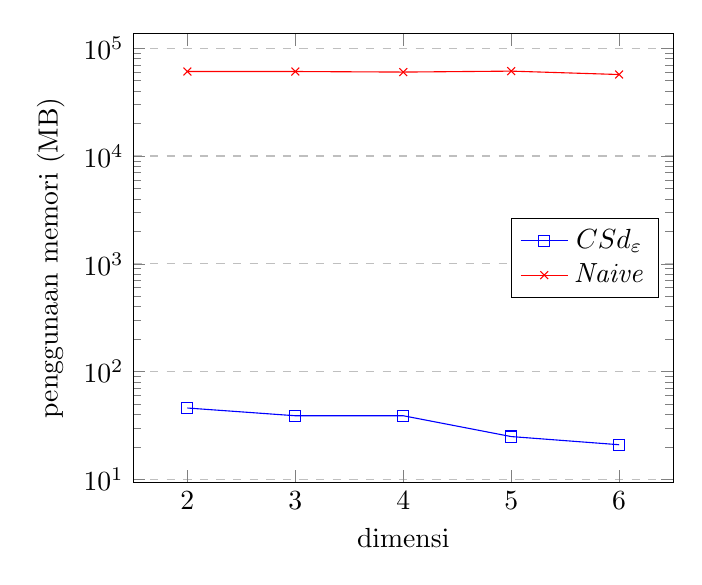
\begin{tikzpicture}
	\begin{axis}[
	xlabel={dimensi},
	ymode=log,
	ylabel={penggunaan memori (MB)},
	xmin=0, xmax=10,
	xtick={1, 3, 5, 7, 9},
	xticklabels={2, 3, 4, 5, 6},
	legend style={at={(0.7,0.5)},anchor=west},
	ymajorgrids=true,
	grid style=dashed,
	]
	
	\addplot[
	color=blue,
	mark=square,
	]
	coordinates {
		(1, 46)(3, 39)(5, 39)(7, 25)(9, 21)
	};
	\addlegendentry{$ CSd_\varepsilon $}
	
	\addplot[
	color=red,
	mark=x,
	]
	coordinates {
		(1, 60714)(3, 60727)(5, 60006)(7, 61235)(9, 56945)
	};
	\addlegendentry{\textit{Naive}}
	
	\end{axis}
	\end{tikzpicture}
	\caption{Pengaruh dimensi terhadap penggunaan memori dalam satuan megabita}\label{fig:uji-dim-mem}
\end{figure}

\subsubsection{Skenario Uji Coba \textit{Performance} Terhadap Jenis Data}
\tab Data \textit{anticorrelated} tidak banyak mempengaruhi komputasi karena pada penghitungan probabilitas \textit{skyline} objek $ X $, tidak banyak objek yang terdapat pada $ PDD(X) $. Dengan data \textit{correlated}, hampir setiap objek $ X $ memiliki objek yang overlap dengan $ PDD(X) $, sehingga proses penghitungan probabilitas \textit{skyline} menjadi lebih lama. Data \textit{independence} tidak berbeda jauh dengan data \textit{anticorrelated} karena objek yang terdapat pada \textit{node} sedikit sehingga tidak banyak objek $ X $ yang memiliki probabilitas \textit{skyline}.

\begin{figure}[H]
	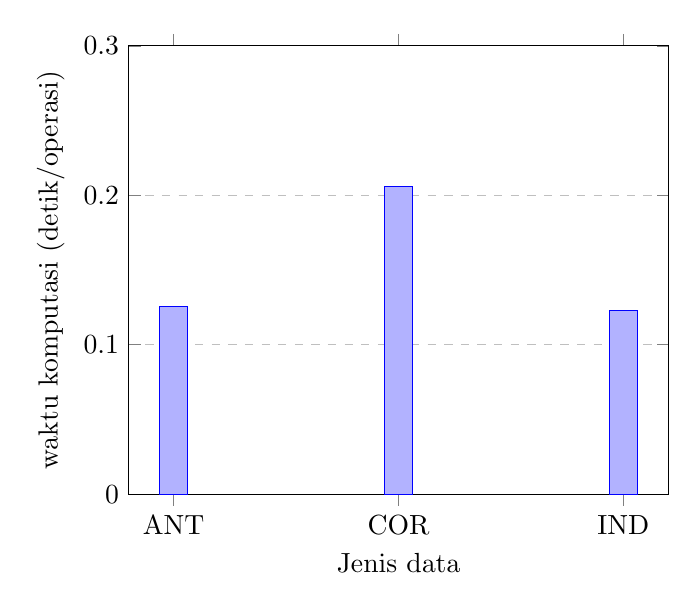
\begin{tikzpicture}
	\begin{axis}[
	ybar,
	ylabel={waktu komputasi (detik/operasi)},
	xlabel={Jenis data},
	symbolic x coords={ANT, COR, IND},
	xtick=data,
	ymin=0, ymax=0.3,
	nodes near coords align={vertical},
	ymajorgrids=true,
	grid style=dashed,
	]
	\addplot 
	coordinates {(ANT, 0.1253)(COR, 0.2059)(IND, 0.1228)};
	\end{axis}
	\end{tikzpicture}
	\caption{Pengaruh jenis data terhadap waktu komputasi tiap operasi dalam satuan detik}\label{GrafikDIND}
\end{figure}


